\chapter{Model Predictive Control Setup}
\label{chapter:MPC}
This chapter presents the setup and creation of the MPC controller and investigates the performance of the resulting controller in the greenhouse environment. Moreover, the effect of the prediction horizon is investigated in nominal and stochastic conditions. The works in this chapter are similar to what is presented in \citet{boersmaRobustSamplebasedModel2022} and \citet{morcegoReinforcementLearningModel2023}. However, direct comparisons are not possible. \citet{boersmaRobustSamplebasedModel2022} develops a robust sample-based controller, where this controller optimises over a number of possible trajectories (due to the parametric uncertainty). While this may produce a policy that will result in lower variance and a higher mean final cumulative reward than a conventional MPC, this chapter will focus on constructing a conventional MPC. This is done to examine the effects of uncertainty on this controller and later asses whether the integration of RL can mitigate these effects. In \citet{morcegoReinforcementLearningModel2023}, such an MPC controller is developed. However, it does not provide specific weather data. Finally, the optimisation goal used in this thesis differs from that in both papers. However, a qualitative comparison may be done.



\section{Greenhouse MPC problem formulation}\label{section: greenhouse MPC formulation}
Similarly to the RL agent, the MPC aims to optimize the objective function defined in \autoref{eq:optimisation-goal}. To facilitate direct comparisons between RL, MPC, and RL-MPC, the same linear penalty constraints, as described in \autoref{eq:penalty_terms}, were used in the form of slack variables. Therefore, the following optimization goal is solved at every time step:

\begin{subequations} \label{eq:mpc_ocp}
	\begin{align}
		\min_{u(k),x(k)} & \sum_{k = k_0}^{k_0 + N_p-1} {l(u(k), y(k))} \\
		\text{s.t.} \quad & x(k+1) = f(x(k), u(k), d(k), \mu_p),  \label{eq:constraint-1} \\
		& y(k) = g(x(k+1), \mu_p), \label{eq:constraint-dynamics} \\
		& -\delta u_{max} \leq u(k) - u(k-1) \leq \delta u_{max}, \label{eq:constraint-delta-u} \\
		& u_{\min} \leq u(k) \leq u_{\max}, \label{eq:constraint-u-limits}\\
		& x(k_0) = x_{k_0}. \label{eq:constraint-initial}\\
	\end{align}
\end{subequations}

This MPC OCP is similar to that discussed in \autoref{ssection:general-mpc}, but it does not include a terminal cost or constraint/region. Furthermore, the constraints are aligned with that of the greenhouse environment. To ensure that the optimisation goal is exactly the same as the RL reward function (\autoref{section:env-description}), the cost function $V(u(k),y(k))$ becomes:

\begin{equation} \label{eq:mpc_stage_cost}
	\begin{aligned}
		l(u(k),y(k)) & = - c_{p_3} (y(k) - y(k-1)) + c_{p_1} u_{1}(k) + c_{p_2} u_{3}(k) + \sum_{i = 1}^6 s_i(k) \\
		\text{where} & \quad s_i(k) \geq 0, \\
		& s_1(k) \geq c_{p_{C02}} \cdot (y_2^{min} - y_2(k)), \\ 
		& s_2(k) \geq c_{p_{C02}} \cdot (y_2(k) + y_2^{max}), \\ 
		& s_3(k) \geq c_{p_{T_{lb}}} \cdot (y_3^{min} - y_3(k)), \\ 
		& s_4(k) \geq c_{p_{T_{ub}}} \cdot (y_3(k) + y_3^{max}), \\ 
		& s_5(k) \geq c_{p_{H}} \cdot (y_4^{min} - y_4(k)), \\ 
		& s_6(k) \geq c_{p_{H}} \cdot (y_4(k) + y_4^{max}), \\
	\end{aligned}	
\end{equation}

The penalty constants $c_{p_{C02}},c_{p_{T_{lb}}},c_{p_{T_{ub}}},c_{p_{H}}$ are the same as those used in the RL problem formulation and given in \autoref{section:env-description}. While MPC can impose hard constraints on the states of the system, which is one of its advantages over RL, it was decided that the same penalty on state violations must be given for a direct comparison between algorithms. Lastly, the policy generated by the MPC is denoted $\kappa(x,u,d,p)$ where the optimal control action to take at time $k$ is

\begin{equation}\label{eq:mpc_policy_notation}
	u(k)^* = \kappa(x(k),u(k-1)^*, d(k), \mu_p)
\end{equation}

It is noted that that with the exception of the current time, the same information is given to both RL and MPC in determining the control input.

\paragraph{Simulation Setup}
Furthermore, the experimental setup is identical to that used in \autoref{section:experimental-setup} except for normalising the states. The performance metrics are the sum of the stage costs (\autoref{eq:mpc_stage_cost}) during the simulation period, equivalent to the EPI minus the sum of the state violations. The performance metric is calculated for the stochastic environment by taking the average of the sum of stage costs over 30 simulation periods and considering the variance of the resulting stage costs. In the case of stochasticity, the MPC algorithm still solves the optimisation problem defined by equation \autoref{eq:mpc_ocp} using the nominal system parameters. However, it is during the system evolution that the uncertainty in parameters is considered. Therefore, a deterministic prediction model is used but the evolution of the state and the output measurements are both uncertain.

Finally, to increase the computational time and feasibility of the MPC solver, the solver is warm-started with the previous solution to reduce the number of iterations required to reach the optimal solution \footnote{The solution to the OCP is heavily reliant on initial guesses due to the non-linearity nature of the problem, lagrangian multipliers from the previous solutions were also reused to mitigate instability in the solver. These instabilities are especially prevalent in longer prediction horizons.}. The computational time of computing the control actions will also be examined for each prediction horizon. These performance metrics are given for all prediction horizons. Finally, the MPC framework is built using the open-source software Casadi \cite{anderssonCasADiSoftwareFramework2019} and the non-linear solver IPOPT \cite{wachterImplementationInteriorpointFilter2006} in python. 

\section{Deterministic Results}
Simulations are conducted for every prediction horizon, $N_p$.The prediction horizons to be tested will include time intervals of 1, 2, 3, 4, 5 and 6 hours. Results include the final cumulative reward and the average time required to solve \autoref{eq:mpc_ocp} for each prediction horizon (averaged across the growing period).

\begin{figure}[H]
	\centering
	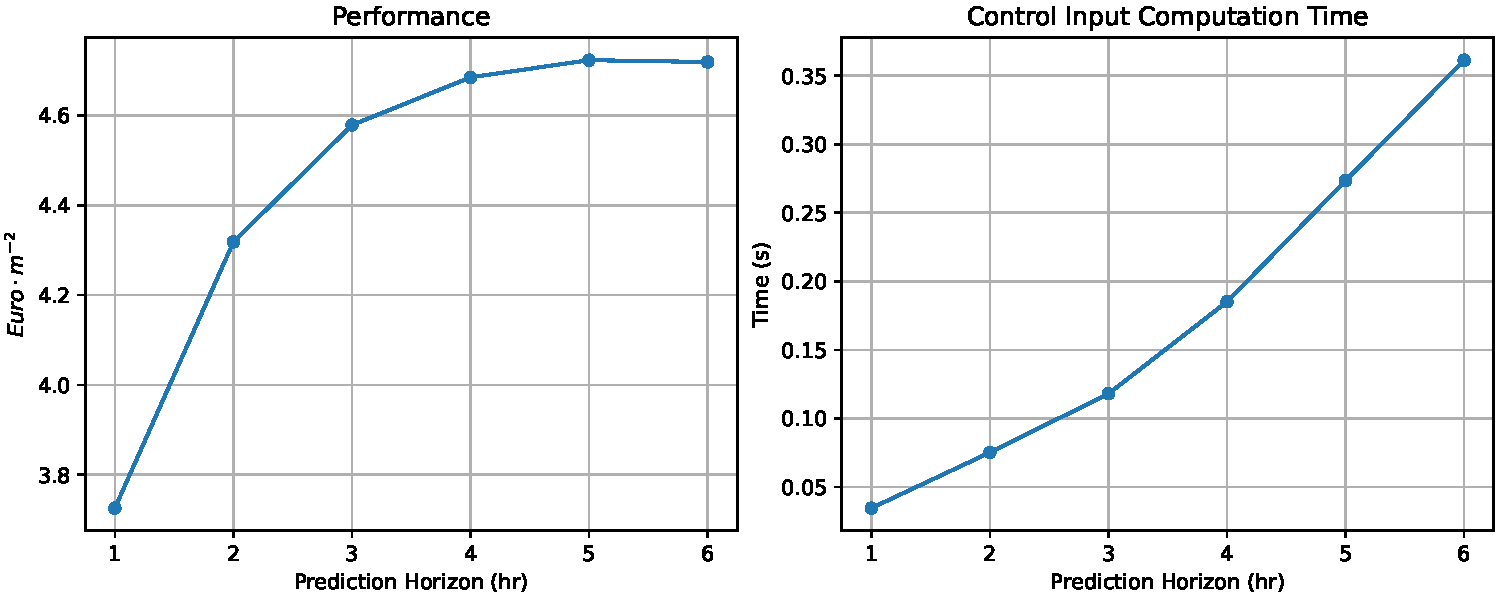
\includegraphics[width=\textwidth]{figures/mpc_nominal.pdf}
	\caption{The final cumulative reward achieved using nominal MPC and the average computation time for each prediction horizon}
	\label{fig:nominal_mpc_perf}
\end{figure}

\autoref{fig:nominal_mpc_perf}  exhibits the performance and the computational time of the MPC for each prediction horizon. It can be seen that performance increases with an increase in prediction horizon up to 6 hours. However, this increase in performance is not guaranteed for an economic model predictive controller as stated in \citet{ellisTutorialReviewEconomic2014}  and \citet{amritEconomicOptimizationUsing2011}. Only with a sufficiently long time horizon or an appropriate terminal cost function or constraints can the performance be guaranteed to increase as the prediction horizon lengthens. Although not entirely clear in \autoref{fig:nominal_mpc_perf}, a prediction horizon of 6 hours produces a slightly lower-performing policy than a prediction horizon of 5 hours. Whether this is due to instabilities in the solver or the nature of the economic optimisation problem remains uncertain.\\
As expected, the computational time in computing the control action increases with an increase in prediction horizon. It is noted that the RL algorithm can calculate the control action in approximately 0.2 milliseconds, while the fastest MPC controller, with a prediction horizon of 1 hour, takes approximately 35 milliseconds, making it 2 order of magnitudes slower. While this outcome is not surprising, it effectively demonstrates the computational demand of MPC, specifically for a highly non-linear model. Nevertheless, setting up and implementing the MPC controller was considerably easier than RL. RL demanded extensive time investment in fine-tuning hyper-parameters. Despite all the fine-tuning in RL, MPC still outperforms the RL agent; this performance difference is analysed in \autoref{chapter:deterministic_RL_MPC}. 
\begin{figure}[H]
	\centering
	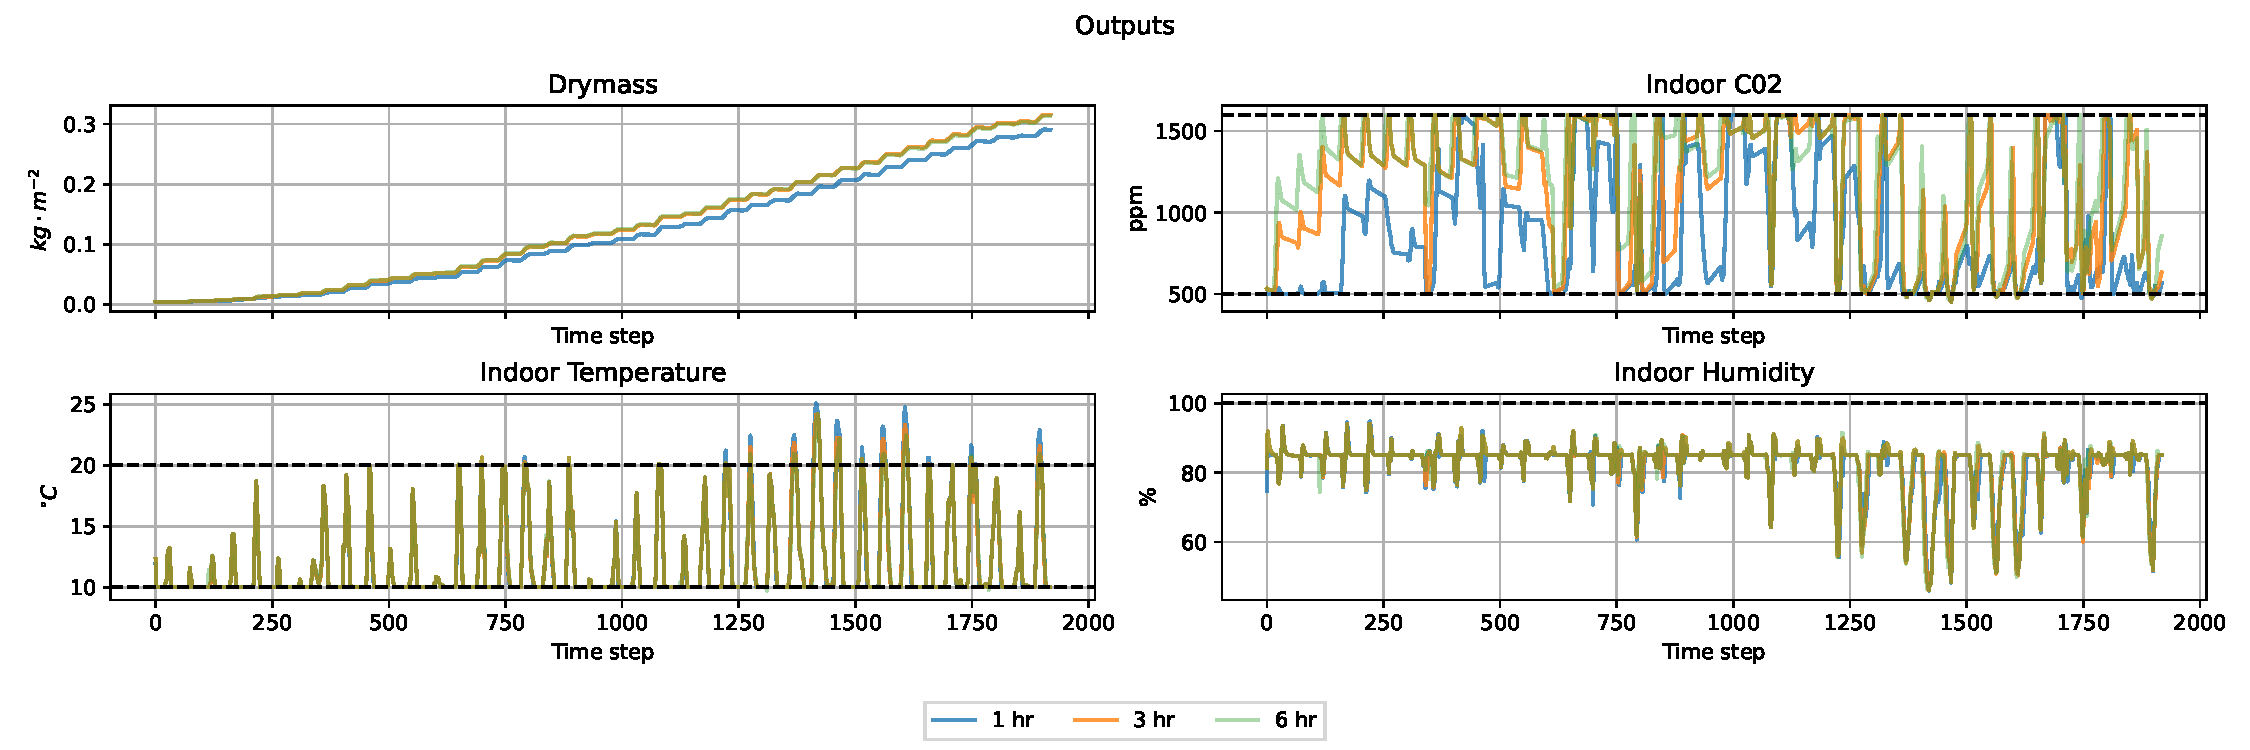
\includegraphics[width=\textwidth]{figures/mpc_outputs_time_series.pdf}
	\caption{MPC 1hr and 5hr Time series of greenhouse outputs}
	\label{fig:mpc-timeseries-outputs}
\end{figure}

\begin{figure}[H]
	\centering
	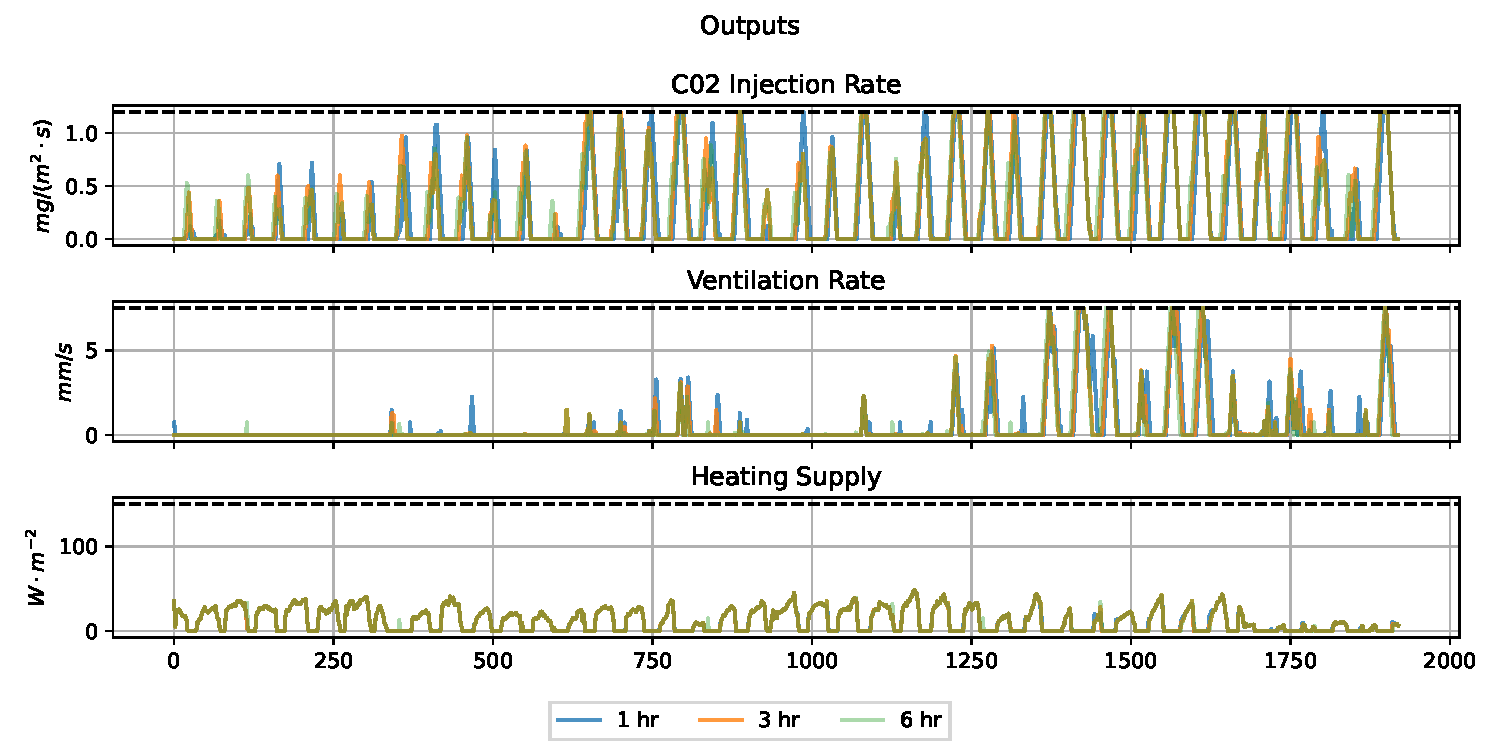
\includegraphics[width=\textwidth]{figures/mpc_inputs_times_series.pdf}
	\caption{MPC 1hr and 5hr time series of controller inputs}
	\label{fig:mpc-timeseries-inputs}
\end{figure}

\autoref{fig:mpc-timeseries-outputs} and \autoref{fig:mpc-timeseries-inputs} display the trajectories of the states and inputs of the best-performing MPC controller (5-hour prediction horizon), the worst-performing (1-hour) and the intermediate controller (3-hour prediction). These are similar trajectories to the RL agents \autoref{fig:selected-policies-outputs} and \autoref{fig:selected-policies-inputs}, respectively. It is noted that, in both cases (RL and MPC), the better-performing policies rapidly raise the indoor C02 levels at the beginning of the growing period by reducing ventilation and increasing C02 injection. However, the trajectories of other states and inputs, particularly the indoor temperature, humidity and heating, appear unchanged. Either the temperature does not play a vital role in plant growth, or the prediction horizon is not long enough to see its effect on the initial growth stages. However, it is clear that the MPC controller uses heating at night and irradiance during the day to ensure that temperature constraints are met. These results are very similar to \citet{morcegoReinforcementLearningModel2023} and \citet{boersmaRobustSamplebasedModel2022}, although difficult to compare quantitatively due to the difference in the optimisation goal and MPC problem formulation.


\section{Stochastic Results}
For each stochastic level, $\delta = 5\%, \delta = 10\%, \delta = 20\%$ were analysed with prediction horizons of 1, 3, and 5 hours. Additional prediction horizons were not considered due to limitations in simulation time.

\begin{figure}[H]
	\centering
	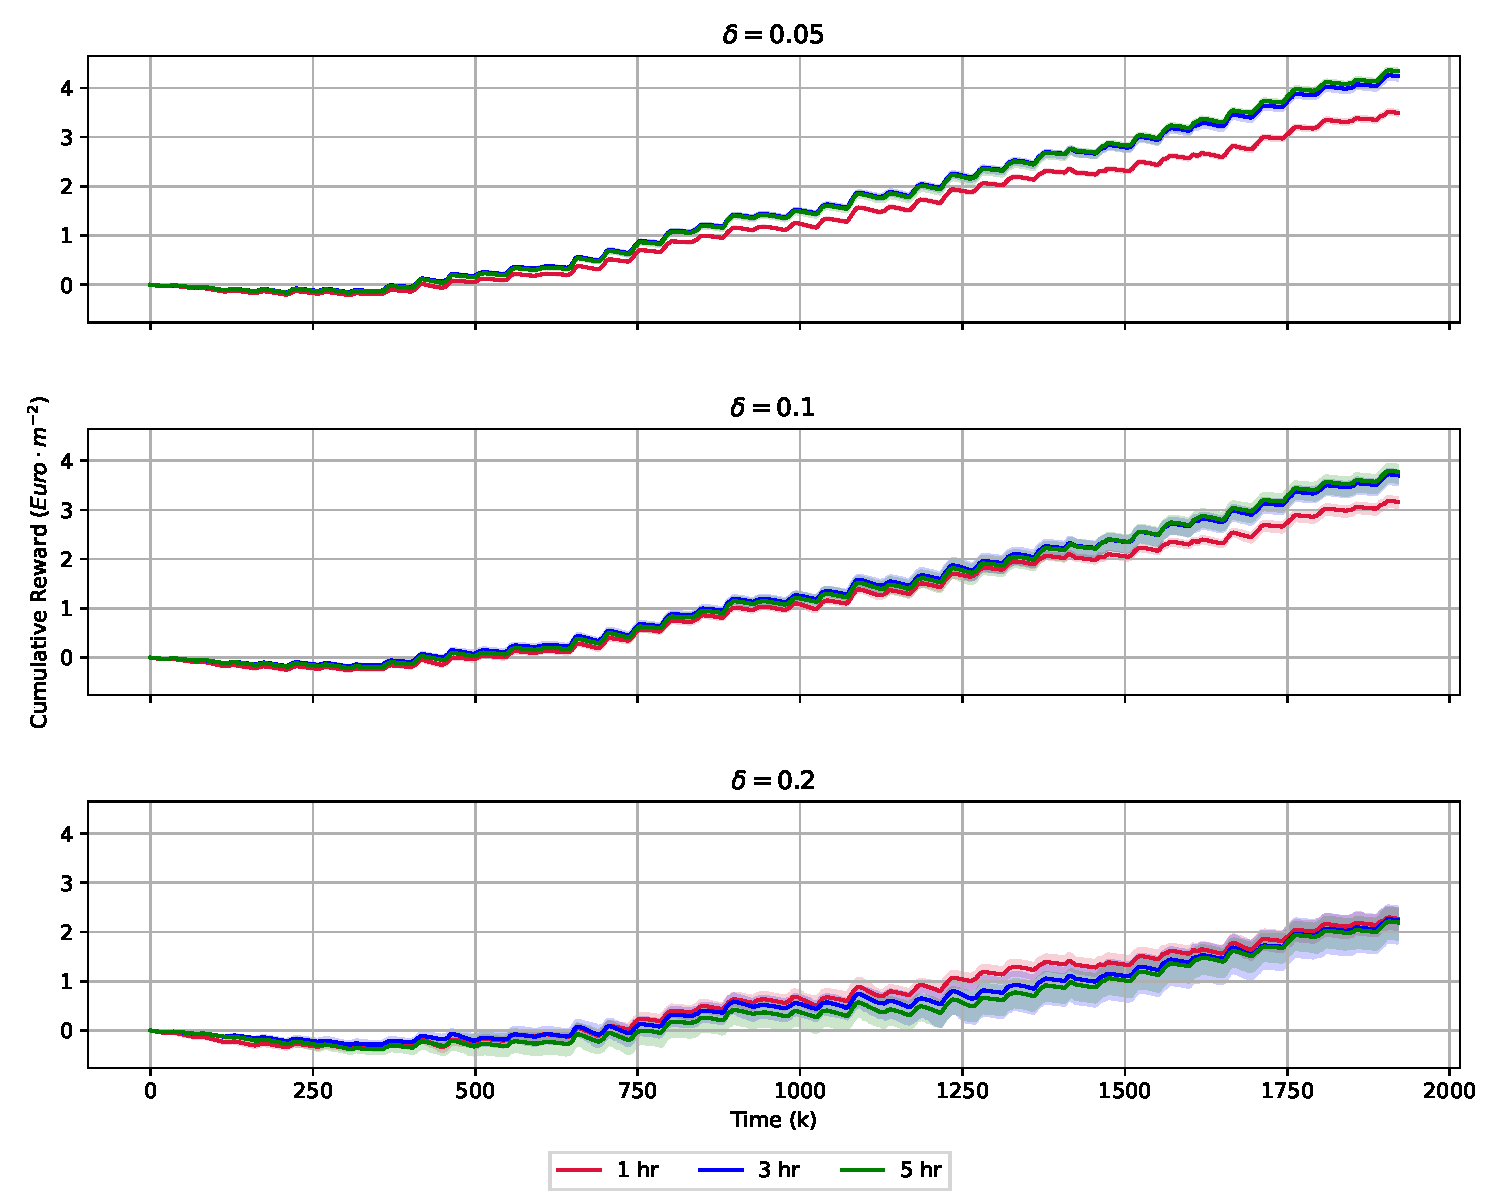
\includegraphics[width=0.8\textwidth]{figures/stochastic_mpc_rewards_time.pdf}
	\caption{Time evolution of cumulative rewards. Displays the evolution of the cumulative reward over the growing period for each stochastic and prediction horizon level. Solid lines represent the mean cumulative reward trajectory with a range indicating the minimum and maximum trajectory recorded in the 30 runs.}
	\label{fig:stochastic-mpc-rewards-time}
\end{figure}

\autoref{fig:stochastic-mpc-rewards-time} shows the impact of introducing uncertainty and its effect on the cumulative reward obtained by the MPC controller at each time step. While a $\delta = 0.05$  does not noticeably impact performance, there is significant performance degradation for $\delta = 0.2$. Also notable is that a longer prediction still results in a higher mean cumulative reward. However, for high uncertainties, specifically $\delta = 0.2$, it seems that a longer prediction horizon has less of an impact on performance, and may even be detrimental in extreme cases of uncertainty.

\begin{figure}[H]
	\centering
	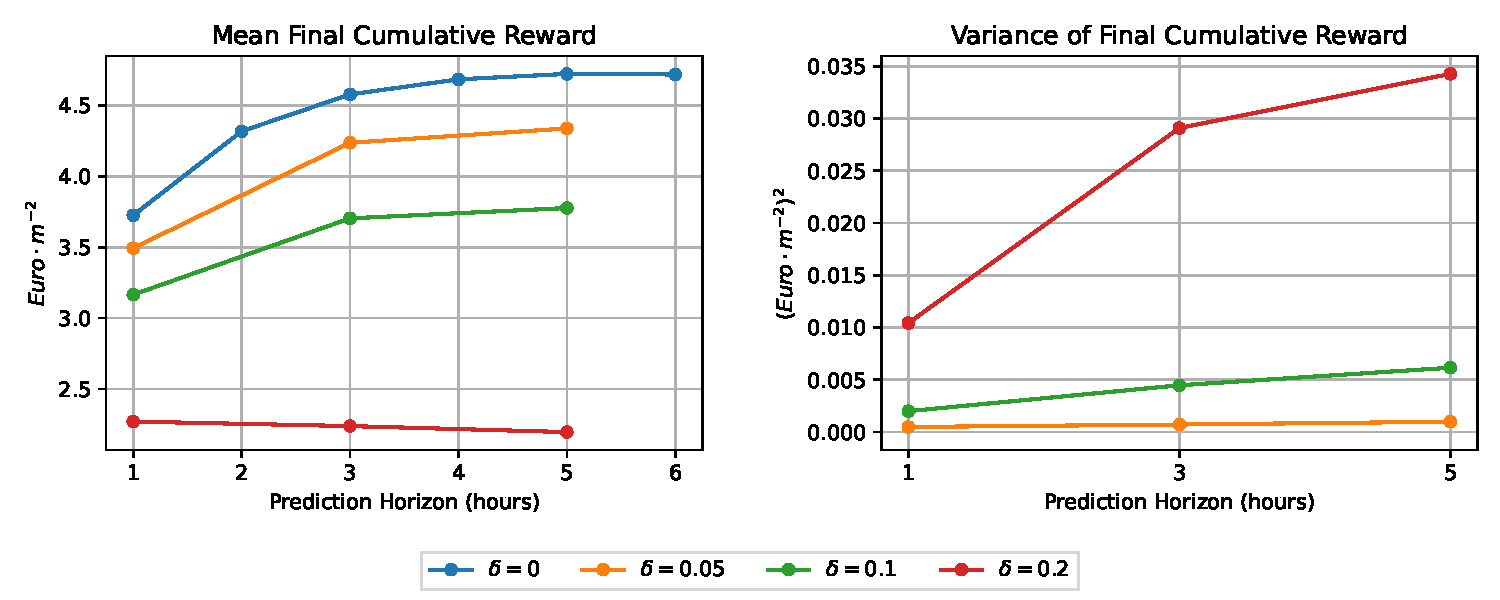
\includegraphics[width=\textwidth]{figures/stochastic_mpc_perf.pdf}
	\caption{MPC performance in stochastic conditions }
	\label{fig:stochastic-mpc-perf}
\end{figure}

\autoref{fig:stochastic-mpc-perf} depicts the final mean and variance values of the cumulative reward for each prediction horizon and uncertainty level, including nominal conditions. \autoref{fig:stochastic-mpc-perf} may provide a better representation of how stochasticity affects the final performance. Increasing the prediction horizon for MPC under higher uncertainty yields diminishing performance returns. Moreover, there is a clear adverse effect on variance as the prediction horizon is increased for all uncertainty levels. This can be attributed to longer prediction horizons becoming progressively less accurate due to the increasing uncertainty of the model parameters. It is acknowledged that a conventional MPC with no knowledge of the uncertainty present is not adept at handling it (although methods such as state estimation exist), and these results confirm this. Although it is possible to formulate a robust MPC, such as in \citet{boersmaRobustSamplebasedModel2022}, it introduces a heavy computational burden on the controller. As previously mentioned, RL’s decrease in performance due to uncertainty is not as drastic as MPC’s as well as the variance in the final cumulative reward is also substantially lower. Thus, it is worth exploring whether the RL agent can assist the MPC in mitigating the adverse impacts of parametric uncertainty.


\section{Conclusion}

In conclusion, this chapter has presented the setup and implementation of the MPC framework whereby the EMPC OCP was designed to maximise the economic advantage of the greenhouse by aligning its optimisation objective with the optimisation goal specified in \autoref{ssection:optimization-goal}. However, additional slack variables were introduced to align the optimisation problem with what the RL agent is optimising for more meaningful comparisons. The MPC controller’s performance was thoroughly examined under nominal and stochastic conditions, focusing on various prediction horizons. The findings and comparisons drawn in this chapter shed light on the controller’s efficacy and limitations in managing a greenhouse environment.

Under deterministic conditions, MPC exhibited varying performance across different prediction horizons. It demonstrated improved economic outcomes with longer prediction horizons, albeit with increased computational demands. However, increasing the prediction horizon does not guarantee an increase in performance without an adequate terminal cost function and/or terminal constraint/region. Notably, while MPC outperforms RL in final cumulative reward under deterministic settings, its computational overhead was significantly higher, highlighting a trade-off between computational efficiency and performance optimisation. The scalability of the computational time is considerably inferior to that of the RL agent. However, it is important to note that it seems that the MPC is not as myopic as original assumed. These short prediction horizons appear to have satisfactorily optimised the greenhouse environment's slow dynamics and sparse rewards. 

Furthermore, stochastic simulations revealed MPC’s vulnerability to uncertainty in the environment. Increasing uncertainty levels adversely affected MPC’s performance, whereby increasing the prediction horizon may become harmful under extreme uncertainty, leading to compromised economic benefits and increased variability in the final cumulative reward. These results underscored MPC’s limited robustness against stochastic influences compared to RL.

In conclusion, while MPC proved effective in deterministic scenarios with appropriate prediction horizons, its performance degradation under stochastic conditions necessitates exploring hybrid RL-MPC strategies to enhance its performance and robustness. Appropriate additions to its formulation must be made to guarantee performance for an EMPC, which the RL agent could potentially solve. 